% 曲线元示意图
\begin{figure}[htbp]
  \centering
  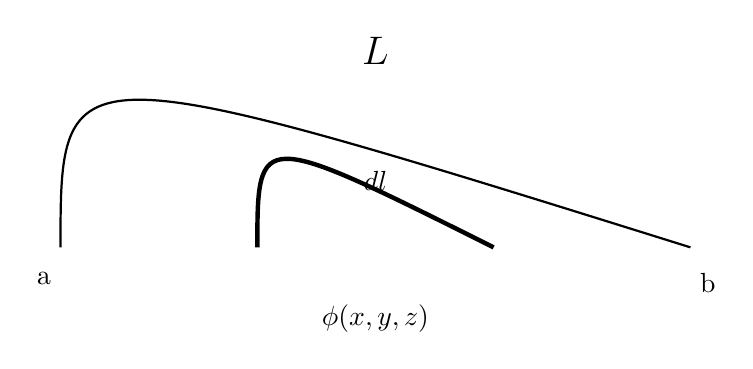
\begin{tikzpicture}[scale=1] % 整体缩放以调整整体大小

    % 1. 绘制背景:一根粗细正常的弧线 (两头有 a, b)
    % 使用贝塞尔曲线,控制点在 (0, 2.5) 处,形成自然的弧度
    \draw[thick] (-4,0) .. controls +(0, 2.5) .. (4,0);

    % 2. 在弧线中间绘制加粗的一段 (上面标注 dl)
    % 只有中间这一段使用 ultra thick
    \draw[ultra thick] (-1.5,0) .. controls +(0, 1.5) .. (1.5,0);

    % 3. 添加文字标注

    % 弧线两端的字母 a 和 b
    \node[below left] at (-4,-0.2) {a};
    \node[below right] at (4,-0.2) {b};

    % 加粗段上方的 dl
    \node[above] at (0, 0.6) {$dl$};

    % 加粗段下方的标量场符号 phi
    \node[below] at (0, -0.6) {$\phi(x,y,z)$};

    % 弧线附近的大写字母 L
    \node[align=center, font=\Large] at (0, 2.5) {$L$};

  \end{tikzpicture}
  \caption{}
  \label{fig:curve-element}
\end{figure}